\documentclass{ali-poster}

\usepackage{lipsum}
\usepackage{graphicx}
\usepackage{ali-macros, ali-pseudocode, ali-crypto}

\title{Balancing Privacy and Accountability on Encrypted Messaging Platforms}
\author{Alistair Pattison and Nick Hopper}
\date{S\&P Oakland, May 2023}

\begin{document}
% 
% ------------------
% -- LEFT PANEL -- 
% ------------------
% 
\noindent%
\begin{panel}{\sidebarwidth}{sidebarcolor}

	\section*{The Protocol}

	This work extends a protocol by Issa, Alhaddad, and Varia called Hecate. In the Hecate protocol, every message requires a token
	\begin{equation*}
		x_1 \ceq \Enc(id_{src}, \ pk_{mod}),
	\end{equation*}
	and an ephemeral key pair $(pk_{eph}, sk_{eph})$. When a user sends a message, she attaches the signature
	\begin{equation*}
		\begin{gathered}
			\sigma_{src} = \Sign_{sk_{eph}}(x_2) \\
			x_2 \ceq x_1 \oplus H(m)
		\end{gathered}
	\end{equation*}
	The signature binds $x_1$ to the sent message, and if the message is ever reported, the moderator decrypts $x_1$ with his private key to obtain the original sender's identity.

	\vspace{2cm}

	% -- PSEUDOCODE -- 
	\begin{algorithmic}[1]
		\function{CreateToken}{$id_{usr}$}{
			\State Compute $x_1 \ceq \tuple{g^r, \ id_{usr} \oplus H(pk_{mod}^r)}$ where $r \gets_\$ \Z_q$
			\State Package $x_1$ into a token and send a signature request to each moderator along with the randomness $r$.
			\State Each moderator verifies verifies $x_1$ and returns their signature share on the token.
			\State Once sufficient responces are recieved, combine the signature shares into into a valid signature.
		}
	\end{algorithmic}

	\vspace{2cm}

	\begin{algorithmic}[1]
		\function{HandleReport}{$m$, $x_1$}{
		\State A coordinator sends a request to all $n$ moderators containing the reported message $m$ and the encrypted id, $x_1 = \tuple{c_1, c_2}$.
		\State If the moderator believes that the message is worth acting upon, she responds with the decrption share $d_i \ceq c_1^{s_i}$.
		\State If enough decryption shares are received, the moderator recovers $x_1$.
		}
	\end{algorithmic}

\end{panel}%
\hspace{\marginwidth}
% 
% ------------------
% -- CENTER PANEL -- 
% ------------------
% 
\begin{panel}{\centerwidth}{white}
	% -- TITLE -- 
	\maketitle

	\vspace{2cm}

	% -- SHORT SUMMARY -- 
	\hfill\parbox{\dimexpr\centerwidth-4cm\relax}{
		\Large
		% TODO input abstract here
		% highlight/bold important sentences
		Encrypted messaging services like WhatsApp, Facebook Messenger, and Signal provide secure and deniable communication for billions across the world, but these exact properties prevent holding users accountable for sending messages that are abusive, misinformative, or otherwise harmful to society.
		This work introduces a protocol in which {\bf\color{highlightcolor} the sender of an abusive message can be identified if there is sufficient agreement among a group of moderators}.
		The protocol {\bf\color{footercolor} retains all security properties of the messaging service for unreported messages}.

	}\hfill\null

	\vspace{2cm}

	% -- NEWSPAPER HEADLINES --
	\begin{center}
		\scalebox{.75}{\parbox{\centerwidth}{
				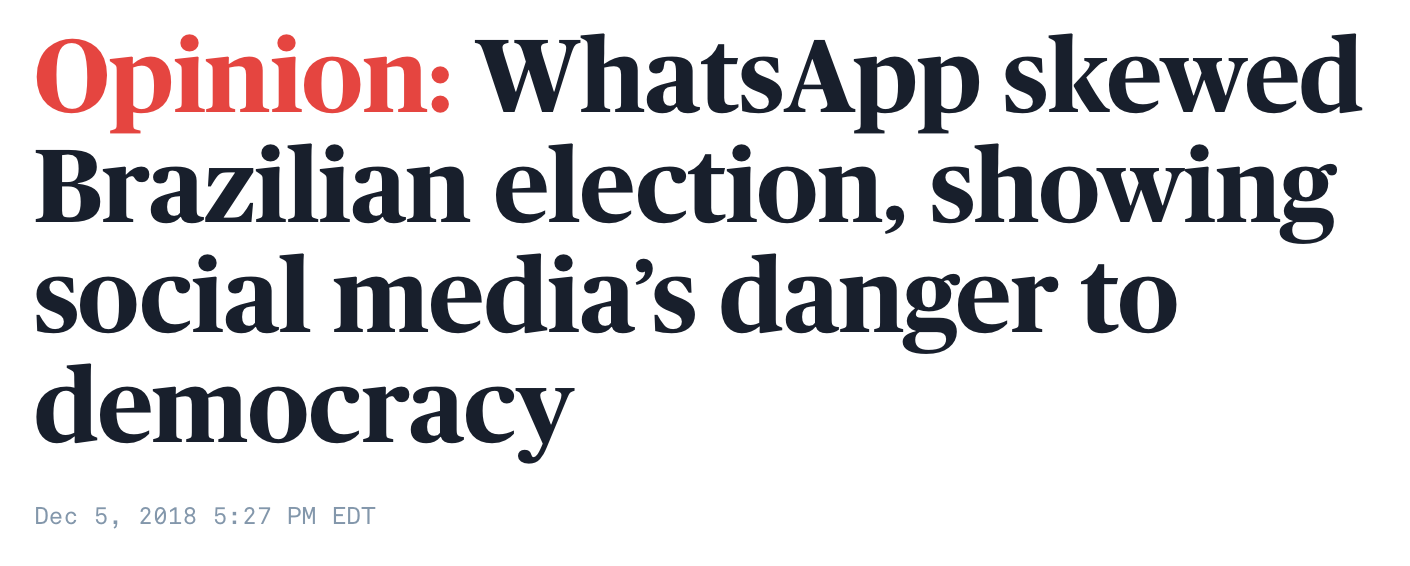
\includegraphics{graphics/brazil-election.png}
				\hspace{2cm}
				
\includegraphics{graphics/india-murder.png}

				\hfill 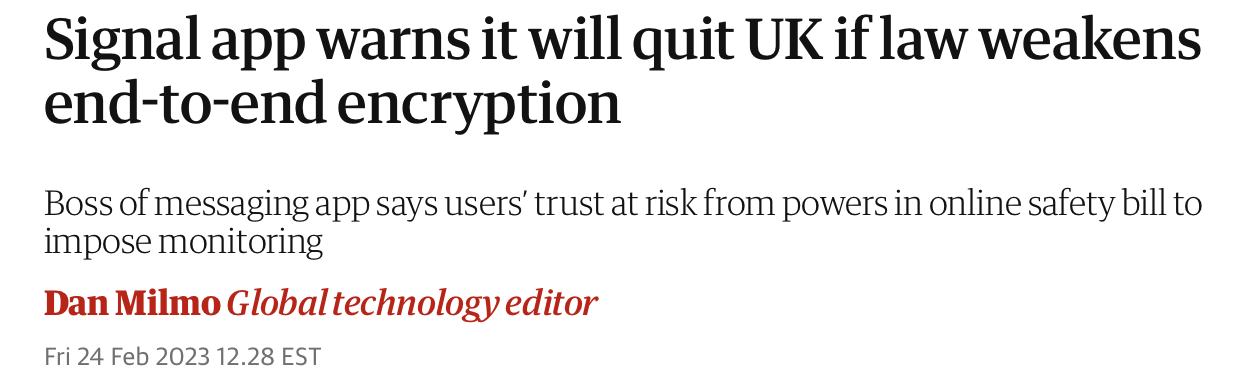
\includegraphics[scale=1.25]{graphics/signal-uk.png} \hfill\null
				\bigskip\bigskip

				\hspace{3cm}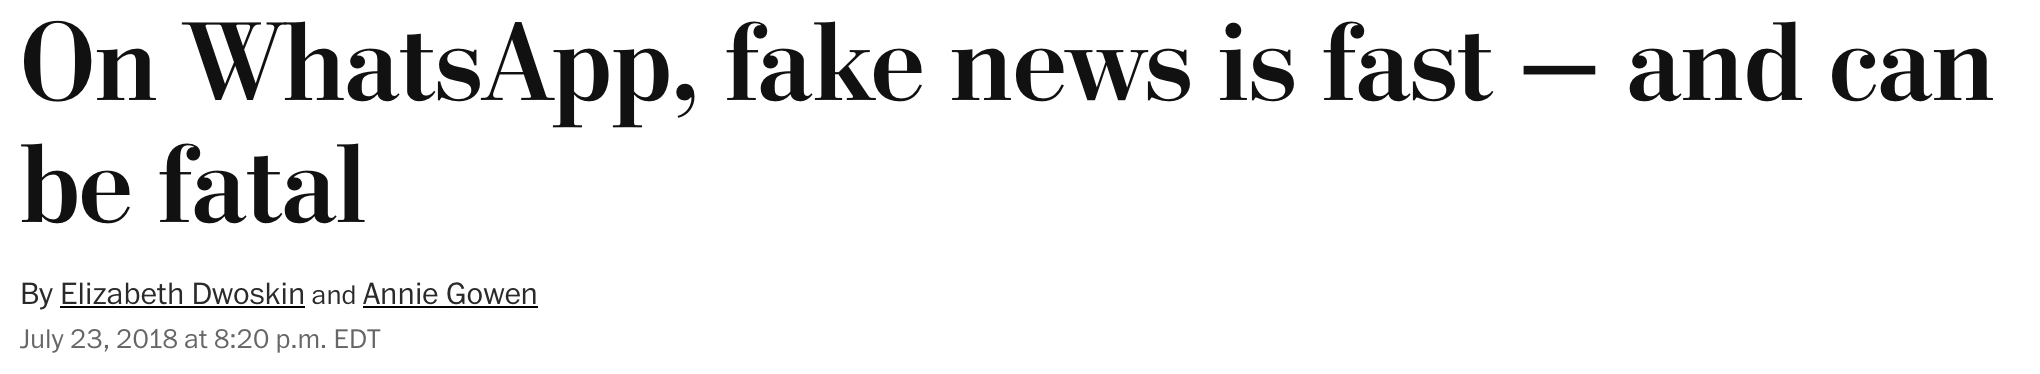
\includegraphics{graphics/fake-news.png}
			}}
	\end{center}

\end{panel}%
\hspace{\marginwidth}
% 
% -------------------
% -- RIGHT PANEL --
% -------------------
% 
\begin{panel}{\sidebarwidth}{sidebarcolor}
	\section*{Benchmarks}

	We implement the protocol in Rust where each party runs in a separate Docker container and communicates over HTTP.

	\vspace{5cm}

	% TODO
	\begin{center}
		\textbf{TO BE COMPLETED FOR \\ FINAL POSTER}
	\end{center}

\end{panel}

\footer{
	\parbox[c][\footerheight]{.5\textwidth}{%
		\Larger \bf
		\ensuremath{\vcenter{\hbox{
					
\includegraphics[height=\dimexpr\footerheight-2cm\relax]{graphics/abstract-qr.png}}
			}}
		% https://www.the-qrcode-generator.com
		\textleftarrow{} Download the extended abstract!
	}%
	\parbox[c][\footerheight]{.5\textwidth}{%
		\hfill
		
\includegraphics[height=\dimexpr\footerheight/3\relax]{graphics/umn-logo.png}
	}
}

\end{document}